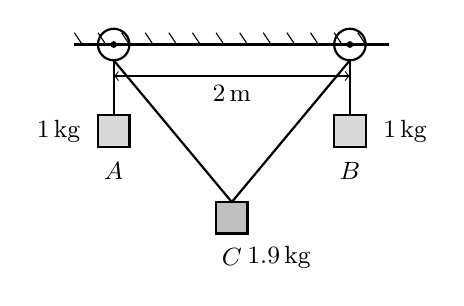
\begin{tikzpicture}[font=\small]
  % 两个等高定滑轮，绳连接A、B，中点挂C
  % 天花板/支架
  \draw[thick] (-2,3.5) -- (2,3.5);
  \foreach \x in {-1.9,-1.6,...,1.9}
    \draw (\x,3.5) -- (\x-0.1,3.65);
  % 左滑轮
  \draw[thick] (-1.5,3.5) circle (0.2);
  \filldraw (-1.5,3.5) circle (1pt);
  % 右滑轮
  \draw[thick] (1.5,3.5) circle (0.2);
  \filldraw (1.5,3.5) circle (1pt);
  % 两滑轮间距
  \draw[<->] (-1.5,3.1) -- (1.5,3.1) node[midway, below] {$2\,\mathrm{m}$};
  % 物块A（左滑轮下方）
  \draw[thick, fill=gray!30] (-1.7,2.2) rectangle (-1.3,2.6);
  \node at (-1.5,1.9) {$A$};
  \draw[thick] (-1.5,3.3) -- (-1.5,2.6);
  % 物块B（右滑轮下方）
  \draw[thick, fill=gray!30] (1.3,2.2) rectangle (1.7,2.6);
  \node at (1.5,1.9) {$B$};
  \draw[thick] (1.5,3.3) -- (1.5,2.6);
  % 绳子中点下垂挂C
  \draw[thick] (-1.5,3.3) -- (0,1.5);
  \draw[thick] (1.5,3.3) -- (0,1.5);
  % 物块C
  \draw[thick, fill=gray!50] (-0.2,1.1) rectangle (0.2,1.5);
  \node at (0,0.8) {$C$};
  % 标注质量
  \node at (-2.2,2.4) {1\,kg};
  \node at (2.2,2.4) {1\,kg};
  \node at (0.6,0.8) {1.9\,kg};
\end{tikzpicture}
